% =====================================================================
%  Chapitre 3 -- Regression et regularisation
%  Partie a : modele lineaire, OLS, diagnostic
% =====================================================================
\section{Chapitre 3 --- Régression et régularisation}

\chapterslide{Chapitre 3}{Régression et régularisation}%
{8 h --- 5 h CM/TD + 3 h TP}%
{\textbf{Objectifs.} Écrire et ajuster un modèle linéaire ; lire ses coefficients ;
diagnostiquer les résidus ; choisir entre OLS, Ridge et Lasso ; régler $\lambda$
par validation croisée.}

\begin{frame}{Prédire un nombre, pas une classe}
\begin{columns}[t]
\begin{column}{0.48\textwidth}
\begin{ebox}[Le problème]
Estimer une quantité continue : loyer, consommation, durée de vie, score
d'examen.
\end{ebox}
\end{column}
\begin{column}{0.48\textwidth}
\begin{kbox}[La différence avec la classification]
La sortie n'est pas une étiquette mais un \textbf{nombre}. Une erreur de 5 et
une erreur de 50 n'ont pas le même poids : la notion de \emph{distance} devient
centrale.
\end{kbox}
\end{column}
\end{columns}
\vspace{2mm}
\begin{solbox}[Le modèle le plus simple qui serve encore]
Une combinaison linéaire des variables d'entrée :
\[
  \hat y = \beta_0 + \beta_1 x_1 + \beta_2 x_2 + \dots + \beta_p x_p
        = \beta_0 + \mathbf{x}^\top\boldsymbol\beta .
\]
\end{solbox}
\end{frame}

\begin{frame}{Ce que dit chaque coefficient}
\begin{center}
\small
\begin{tabular}{@{}p{0.20\textwidth}p{0.30\textwidth}p{0.40\textwidth}@{}}
\toprule
\textbf{Paramètre} & \textbf{Nom} & \textbf{Lecture} \\
\midrule
$\beta_0$ & ordonnée à l'origine & valeur prédite quand toutes les variables
sont nulles \\
$\beta_j$ & coefficient & variation de $\hat y$ quand $x_j$ augmente de
\textbf{une unité}, les autres variables étant fixées \\
\bottomrule
\end{tabular}
\end{center}
\vspace{2mm}
\begin{wbox}[La phrase à savoir prononcer]
« Toutes choses égales par ailleurs, une unité de plus sur $x_j$ change la
prédiction de $\beta_j$. » Sans le « toutes choses égales », la phrase est fausse.
\end{wbox}
\end{frame}

\begin{frame}{Ajuster : minimiser les carrés}
\begin{columns}[t]
\begin{column}{0.50\textwidth}
On cherche $\boldsymbol\beta$ qui minimise
\[
  \hat R_n(\boldsymbol\beta)=\frac{1}{n}\sum_{i=1}^{n}\big(y_i-\hat
  y_i\big)^2 .
\]
C'est la \textbf{méthode des moindres carrés ordinaires} (OLS).

\vspace{1mm}
Sa solution, quand $X^\top X$ est inversible :
\[
  \hat{\boldsymbol\beta}=(X^\top X)^{-1}X^\top y .
\]
\end{column}
\begin{column}{0.46\textwidth}
\begin{kbox}[Pourquoi le carré ?]
Il pénalise davantage les grosses erreurs, il est dérivable partout, et il
correspond à un bruit gaussien.
\end{kbox}
\begin{wbox}[Quand $p$ dépasse $n$]
$X^\top X$ n'est plus inversible : une infinité de solutions. C'est là que la
régularisation devient nécessaire.
\end{wbox}
\end{column}
\end{columns}
\end{frame}

\begin{frame}{Sur données réelles : le diabète}
\begin{columns}[t]
\begin{column}{0.52\textwidth}
\centering
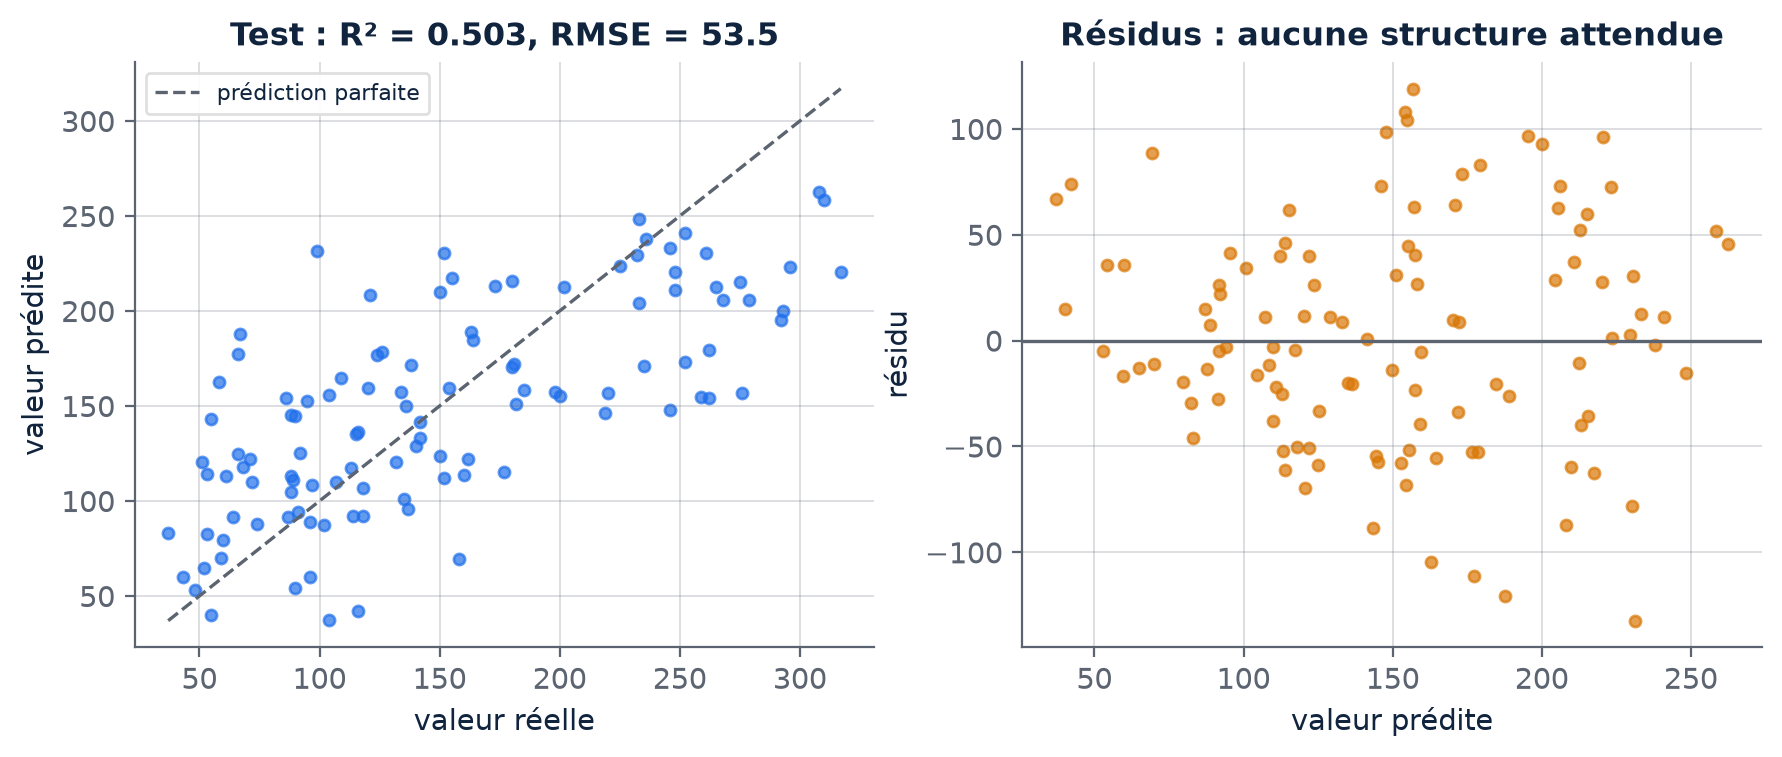
\includegraphics[height=0.34\textheight,keepaspectratio]{k01_ajustement.png}
\end{column}
\begin{column}{0.44\textwidth}
\begin{itemize}
  \item 442 patients, 10 variables cliniques.
  \item Entraînement : 331 ; test : 111.
  \item OLS : $R^2=\mathbf{0{,}503}$, RMSE $=\mathbf{53{,}5}$,
        MAE $=\mathbf{43{,}4}$.
\end{itemize}
\begin{kbox}[Lecture]
Le modèle explique la moitié de la variance. Ce n'est ni excellent ni nul :
c'est le niveau réel de ce jeu, et une baseline honnête.
\end{kbox}
\end{column}
\end{columns}
\end{frame}

\begin{frame}{Quatre hypothèses, et ce qu'elles impliquent}
\begin{center}
\small
\begin{tabular}{@{}p{0.20\textwidth}p{0.34\textwidth}p{0.36\textwidth}@{}}
\toprule
\textbf{Hypothèse} & \textbf{Énoncé} & \textbf{Violation : conséquence} \\
\midrule
Linéarité & $y$ est linéaire en $x$ & biais systématique, résidus en motif \\
Indépendance & les erreurs ne se répètent pas & intervalles et tests invalides \\
Homoscédasticité & variance constante & coefficients non optimaux, tests faux \\
Normalité & erreurs gaussiennes & utile pour les tests, pas pour prédire \\
\bottomrule
\end{tabular}
\end{center}
\vspace{2mm}
\begin{kbox}[À retenir]
Ces hypothèses concernent les \textbf{erreurs}, pas les variables. On les vérifie
sur les \textbf{résidus}, après ajustement.
\end{kbox}
\end{frame}

\begin{frame}{Lire les résidus}
\begin{columns}[t]
\begin{column}{0.48\textwidth}
\centering
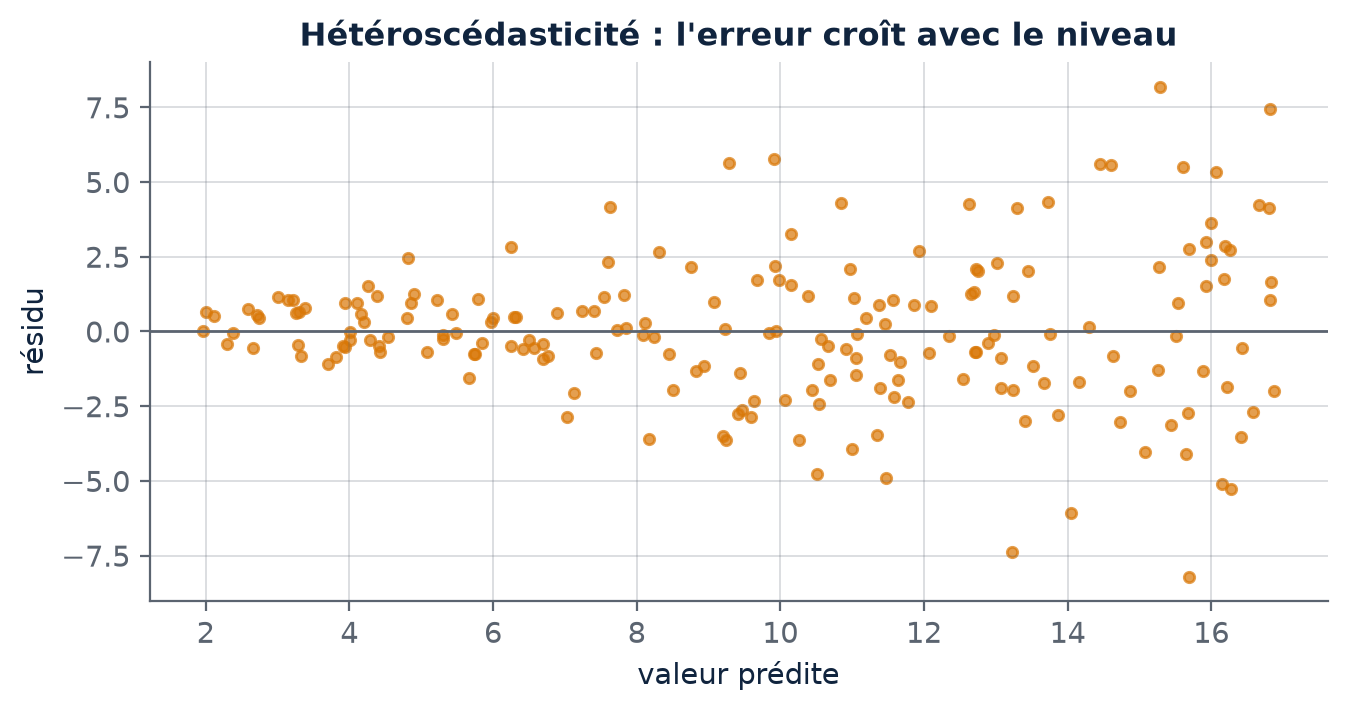
\includegraphics[height=0.32\textheight,keepaspectratio]{k06_heteroscedasticite.png}
\end{column}
\begin{column}{0.50\textwidth}
\begin{itemize}
  \item Résidus en entonnoir : la variance croît avec la prédiction.
  \item Mesure : corrélation entre $|\text{résidu}|$ et $\hat y$ :
        \textbf{0,508} ici.
  \item Un motif courbe signale une non-linéarité.
  \item Un point isolé très loin : influence à examiner.
\end{itemize}
\begin{wbox}[Ce que l'on attend]
Un nuage sans structure, centré sur zéro, de largeur constante.
\end{wbox}
\end{column}
\end{columns}
\end{frame}

\begin{frame}{Corrélation n'est pas régression}
\begin{columns}[t]
\begin{column}{0.48\textwidth}
\begin{ebox}[Ce que donne la corrélation]
Un seul nombre, entre $-1$ et $1$, qui mesure l'intensité d'une relation
\emph{linéaire} entre deux variables.
\end{ebox}
\end{column}
\begin{column}{0.48\textwidth}
\begin{ebox}[Ce que donne la régression]
Un coefficient par variable, qui isole l'effet de chacune \textbf{à niveau des
autres constant}.
\end{ebox}
\end{column}
\end{columns}
\vspace{2mm}
\begin{wbox}[Deux pièges]
Une corrélation nulle n'exclut pas une relation en U. Et une corrélation forte
entre $x_1$ et $x_2$ ne dit rien sur le coefficient de $x_1$ dans un modèle
multiple.
\end{wbox}
\end{frame}

\begin{frame}{La liste de contrôle du diagnostic}
\begin{enumerate}
  \item \textbf{Linéarité} : les résidus dessinent-ils un motif ?
  \item \textbf{Homoscédasticité} : l'épaisseur du nuage est-elle constante ?
  \item \textbf{Points influents} : un point isolé tire-t-il la droite ?
  \item \textbf{Colinéarité} : deux variables portent-elles la même information ?
  \item \textbf{Fuite} : une variable est-elle connue après la décision ?
\end{enumerate}
\vspace{1.5mm}
\begin{kbox}[Un défaut trouvé vaut mieux que dix scores]
Un $R^2$ élevé avec des résidus en U annonce un modèle qui se trompera
systématiquement sur une partie du domaine.
\end{kbox}
\end{frame}

\begin{frame}{Trois indicateurs, trois lectures}
\begin{center}
\small
\begin{tabular}{@{}p{0.16\textwidth}p{0.34\textwidth}p{0.40\textwidth}@{}}
\toprule
\textbf{Indicateur} & \textbf{Formule} & \textbf{Quand il trompe} \\
\midrule
$R^2$ & $1-\dfrac{\sum (y_i-\hat y_i)^2}{\sum (y_i-\bar y)^2}$ & augmente avec le
nombre de variables, même inutiles \\
RMSE & $\sqrt{\frac1n\sum (y_i-\hat y_i)^2}$ & dominée par les grosses erreurs \\
MAE & $\frac1n\sum |y_i-\hat y_i|$ & sous-estime le coût des erreurs extrêmes \\
\bottomrule
\end{tabular}
\end{center}
\vspace{2mm}
\begin{kbox}[Sur le jeu du diabète]
RMSE $53{,}5$ et MAE $43{,}4$ : l'écart indique des erreurs inégales. Le $R^2$
seul ne dit pas cela.
\end{kbox}
\end{frame}

\begin{frame}{Activité 1 --- interpréter (8 min)}
\begin{abox}[Un modèle de loyer]
$\hat y = 15{,}2 + 0{,}42\,x_{\text{surface}} - 1{,}8\,x_{\text{étage}}$
(où $y$ est en milliers de FCFA).
\begin{enumerate}
  \item Que signifie $0{,}42$ ?
  \item Que signifie $-1{,}8$ ? Est-ce plausible ?
  \item Prédire le loyer pour 60 m$^2$ au 3\textsuperscript{e} étage.
\end{enumerate}
\end{abox}
\vspace{1mm}
\begin{solbox}[Réponses]
\textbf{1.} +420 FCFA par m$^2$ supplémentaire, à étage constant.
\textbf{2.} $-1{,}8$ millier par étage : le modèle suppose que monter fait
baisser le loyer — à vérifier, cela peut signaler un effet mal spécifié.
\textbf{3.} $15{,}2+0{,}42\times60-1{,}8\times3=\mathbf{35{,}0}$ milliers.
\end{solbox}
\end{frame}

\begin{frame}{Multicolinéarité : des coefficients qui mentent}
\begin{columns}[t]
\begin{column}{0.46\textwidth}
\centering
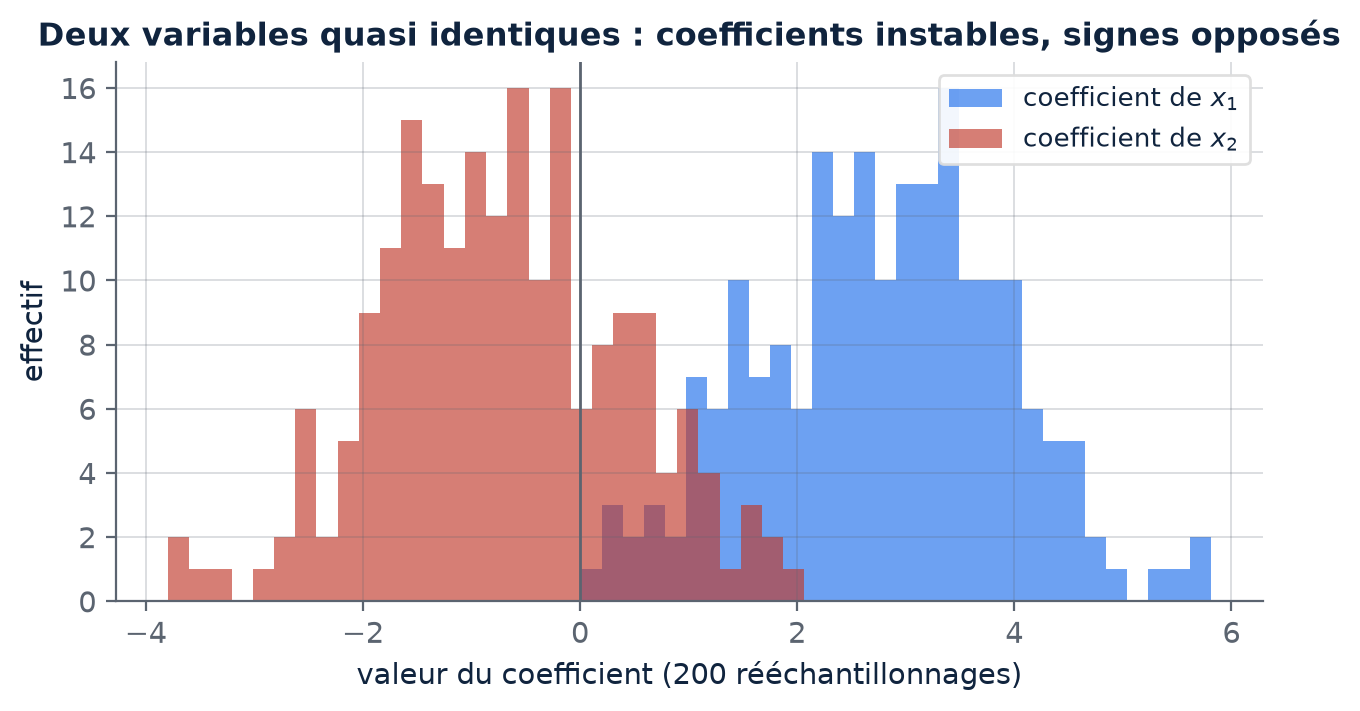
\includegraphics[height=0.32\textheight,keepaspectratio]{k07_multicolinearite.png}
\end{column}
\begin{column}{0.52\textwidth}
\begin{itemize}
  \item Deux variables corrélées à \textbf{0,999}.
  \item Sur 200 rééchantillonnages : coefficient de $x_1$ =
        $2{,}76 \pm 1{,}13$ ; coefficient de $x_2$ = $-0{,}73 \pm 1{,}12$.
  \item Les signes s'inversent d'un échantillon à l'autre.
\end{itemize}
\begin{wbox}[Conséquence]
La prédiction reste correcte, mais \textbf{l'explication est inutilisable} :
impossible de dire quelle variable agit.
\end{wbox}
\end{column}
\end{columns}
\end{frame}

\begin{frame}{Quiz 1 --- modèle linéaire}
\begin{columns}[t]
\begin{column}{0.49\textwidth}
\begin{qbox}[Question 1]
Le coefficient $\beta_j$ mesure :
\begin{itemize}
  \item[(a)] la corrélation entre $x_j$ et $y$
  \item[(b)] la variation de $\hat y$ pour une unité de plus sur $x_j$
  \item[(c)] l'importance absolue de $x_j$
\end{itemize}
\end{qbox}
\begin{qbox}[Question 2]
Le $R^2$ augmente si l'on ajoute :
\begin{itemize}
  \item[(a)] une variable utile \quad (b) une variable inutile
  \item[(c)] les deux
\end{itemize}
\end{qbox}
\end{column}
\begin{column}{0.49\textwidth}
\begin{qbox}[Question 3]
Un résidu en entonnoir signale :
\begin{itemize}
  \item[(a)] une non-linéarité
  \item[(b)] une variance non constante
  \item[(c)] une variable manquante
\end{itemize}
\end{qbox}
\begin{solbox}[Réponses]
\textbf{1.} (b). \quad \textbf{2.} (c) : le $R^2$ ne décroît jamais.
\quad \textbf{3.} (b).
\end{solbox}
\end{column}
\end{columns}
\end{frame}
